\documentclass{beamer}
\usepackage{amsmath}%
\usepackage{amsfonts}%
\usepackage{amssymb}%
\usepackage{amsthm}%
\usepackage{graphicx}
\graphicspath{ {./Figures/} }
%\usepackage{hyperref}

\usepackage{graphicx}
\usepackage{subfig}

\usepackage[czech]{babel}
\usepackage[utf8]{inputenc}

\usepackage{multicol}
%\usepackage{natbib}%
\usepackage{units}

\usepackage{stmaryrd}
\usepackage{gensymb}
\usepackage{bibentry}
\usepackage{accents}

%\usepackage{booktabs}

\usepackage{tensor}
\usepackage[bbgreekl]{mathbbol}
\usepackage{bm}
\usepackage{ulem}

% FANCY TABLES
\usepackage{booktabs}
\usepackage{multirow}
\usepackage{threeparttable}

%\usetheme{Luebeck}
\usetheme{Madrid}
%\usetheme{CambridgeUS}
%\usetheme{Pittsburgh}
%\usetheme{default}
%\mode<presentation>

%FOR CAMBRIDGE US THEME -- red bullets/captions in itemize environment
\setbeamercolor{item projected}{bg=black}
\setbeamertemplate{enumerate items}[default]
\setbeamertemplate{navigation symbols}{}
\setbeamercovered{transparent}

\setbeamercolor*{enumerate item}{fg=black}
\setbeamercolor*{enumerate subitem}{fg=black}
\setbeamercolor*{enumerate subsubitem}{fg=black}

\setbeamercolor{block title}{fg=black}
\setbeamercolor{caption name}{fg=black}

\title[Mechanika]{Inverzné Kyvadlo}
\author[Skupina Z] {Marek Mikloš, Ondřej Kureš, Ladislav Trnka \\ }
\institute[Charles University]{Charles University, Czech Republic}
\date{\today}




\let\newblock\relax

\newcommand{\smallbibentry}[1]{{\tiny \bibentry{#1}}}

% \AtBeginSection[]
% {
%   \begin{frame}
% %    \frametitle{Outline}
%     \tableofcontents[currentsection]
%   \end{frame}
% }

\begin{document}

\begin{frame}
\titlepage

\end{frame}

% \begin{frame}
%   \frametitle{Outline}
%   \tableofcontents
% \end{frame}

\section*{Inverzné Kyvadlo}
\label{sec: Int}


\begin{frame}
 
\frametitle{Inverzné Kyvadlo}


\begin{center}
Cart and pole apparatus, tiltmeter, Kapitza's pendulum.\\    
Lagrangeov pohľad.\\
\end{center}
\begin{small}
\begin{align*}
\mathcal{L} & \stackrel{\text{def}}{=} T-V  \\
\mathcal{L} & =  \frac{1}{2} m \left( l^{2} \left( \frac{\mathrm{d}\theta}{\mathrm{d}t}\right)^{2}+\left( \frac{\mathrm{d}\xi}{\mathrm{d}t}\right)^{2}+2l \sin \theta \frac{\mathrm{d}\xi}{\mathrm{d}t}  \frac{\mathrm{d}\theta}{\mathrm{d}t} \right) -mg \left( \xi-l \cos \theta \right) \\
\end{align*}
Pohybová rovnice:
\begin{align*}
 -\frac{\mathrm{d}}{\mathrm{d}t} \left(  \frac{\partial\mathcal{L}}{\partial\dot{q_{i}}} \right) + \frac{\partial\mathcal{L}}{\partial q_{i}}  & = 0 \\
\frac{\mathrm{d}^{2}\theta}{\mathrm{d} t^{2}}+\left(  \frac{g}{l}-\frac{A \Omega^{2}}{l} \cos \Omega t \right)   \sin \theta &= 0 \\
\end{align*}
\end{small}

\end{frame}

\begin{frame}

\frametitle{Inverzné Kyvadlo}
\begin{center}
Mathieuho rovnica.\\
Perturbačná metóda určenia hraníc, $\alpha, \beta$.\\
\end{center}

\begin{small}
Linearizovaná rovnice:
\begin{equation*}
\frac{\mathrm{d}^{2}\theta}{\mathrm{d} t^{2}}+\left(  \frac{g}{l}-\frac{A \Omega^{2}}{l} \cos \Omega t \right)   \theta =0
\end{equation*}
Přeznačení - parametry:
\begin{align*}
t^{\star} & \stackrel{\text{def}}{=} \Omega t \\
\alpha & \stackrel{\text{def}}{=} \frac{\omega^{2}_{0}}{\Omega^{2}} \\
\beta & \stackrel{\text{def}}{=} -\frac{A}{l} \\
\end{align*}
Mathieu rovnica:
\begin{equation*}
\frac{\mathrm{d}^{2}\theta^{\star}}{\mathrm{d} t^{\star}^{2}}+\left( \alpha + \beta \cos t^{\star} \right)   \theta^{\star} =0
\end{equation*}

\end{small}



\end{frame}
 

\section*{Záver}
\label{sec:Záver}

\begin{frame}
\frametitle{Inverzné Kyvadlo}


\begin{figure}
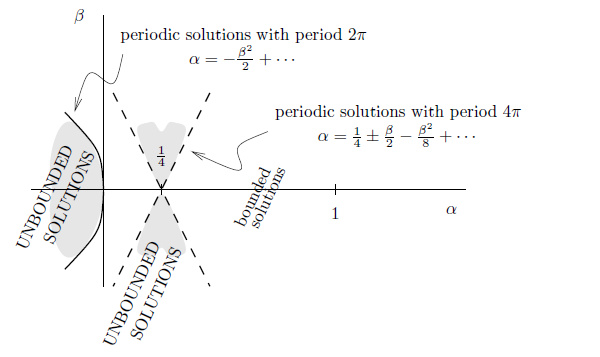
\includegraphics[scale=0.45]{Boundary-graph.png}
\end{figure}

\begin{small}

\begin{itemize}
\item Ak sú hodnoty parametrov $\alpha$ a $\beta$ z tmavej oblasti so stredom v bode $\alpha=\frac{1}{4}$, potom môže byť kyvadlo destabilizované osciláciou pivotu.
\item Pre vhodne zvolené hodnoty parametrov $\alpha$, $\beta$ dosiahneme stabilizáciu kyvadla v hornej časti pri splnenej nutnej podmienke stability (pri zápornom $\alpha$):
\end{itemize}

\begin{equation*}
\frac{A}{l}\frac{\Omega}{\omega_0}\geq \sqrt{2}.
\end{equation*}  
\end{small}


 

\end{frame}

\begin{frame}
\frametitle{Numerická aproximace}

\begin{figure}
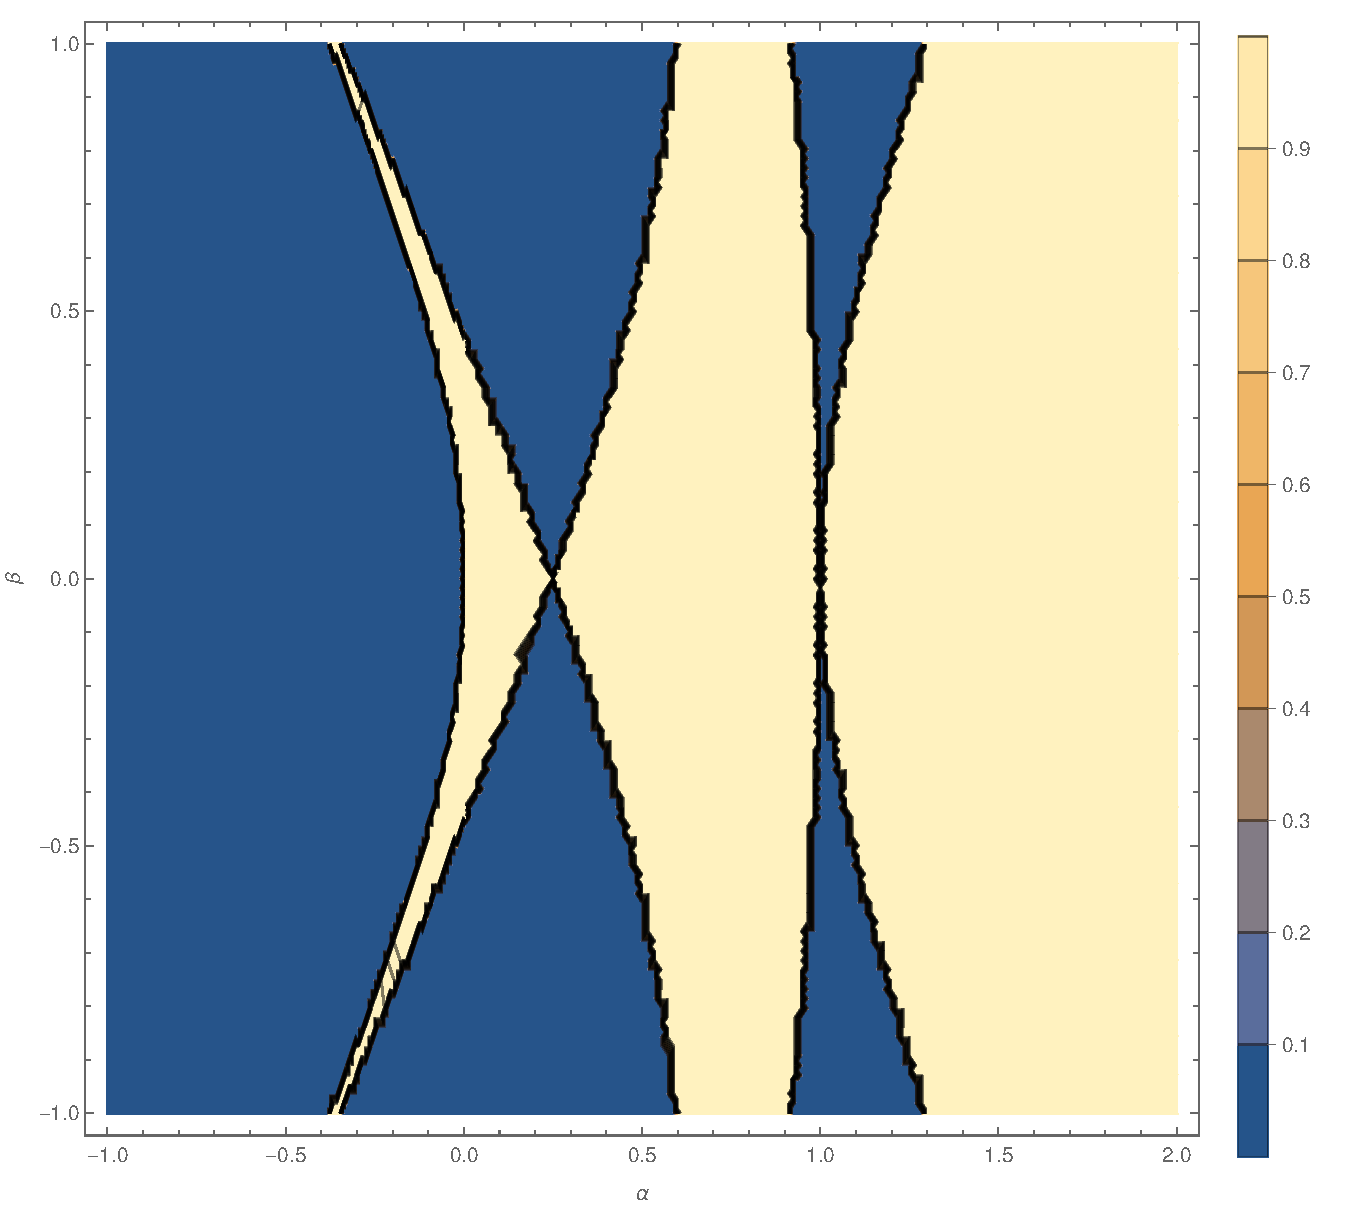
\includegraphics[scale=0.34]{Figure2_num.pdf}
\end{figure}
\begin{center}
\begin{tiny}
Numerická aproximace oblastí s neomezeným řešením (modrá) a omezeným řešením (žlutá).
\end{tiny}
\end{center}


\end{frame}


\end{document}

%
%
%
%
% DOCUMENT ENDS HERE
%
%
%
%
